% ------------
% --------------------

\newpage
\section{REST}
\newpage


\begin{minted}[bgcolor=LightGray,fontsize=\footnotesize,breaklines]{python}
# Wie sind die Ladesäulen in den USA geografisch verteilt

map_center = [stations['Latitude'].mean(), stations['Longitude'].mean()]
my_map = folium.Map(location=map_center, zoom_start=5)
heat_data = [[row['Latitude'], row['Longitude']] for index, row in stations.iterrows()]
HeatMap(heat_data).add_to(my_map)
#HeatMap(heat_data, radius=15, blur=10).add_to(my_map)
my_map
\end{minted}

\begin{center}
\includegraphics[scale=0.2]{img/WhatsApp Image 2023-12-02 at 15.58.19.jpeg}
\end{center}

\begin{minted}[bgcolor=LightGray,fontsize=\small,breaklines]{python}
# Welche Bundestaaten haben die höchste bzw. niedrigste Anzahl an Ladesäulen

stations_per_state = stations.groupby('State').size().reset_index(name='Count')

plt.figure(figsize=(10,5))
plt.bar(stations_per_state['State'], stations_per_state['Count'])
plt.xlabel('US Bundesstaaten')
plt.ylabel('Ladesäulen')
plt.xticks(rotation='vertical')
plt.title('Anzahl an Ladesäulen')
plt.show()
\end{minted}

\begin{center}
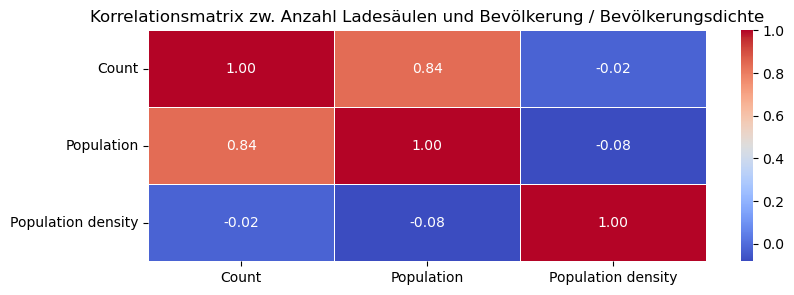
\includegraphics[scale=0.6]{img/output_7_0.png}
\end{center}

\begin{minted}[bgcolor=LightGray,fontsize=\small,breaklines]{python}
# Wie hat sich die Anzahl der Ladesäulen im Laufe der Zeit entwickelt

stations_dev = stations.groupby(stations['Open Date'].dt.date).size().cumsum().reset_index(name='Count')

plt.figure(figsize=(10,5))
plt.plot(stations_dev['Open Date'], stations_dev['Count'], marker='o', linestyle='-')
plt.title('Kumulative Anzahl der Ladesäulen über die Zeit')
plt.xlabel('Datum')
plt.ylabel('Kumulative Anzahl der Ladesäulen')
plt.show()
\end{minted}

\begin{center}
\includegraphics[scale=0.6]{img/output_9_0.png}
\end{center}

\begin{minted}[bgcolor=LightGray,fontsize=\small,breaklines]{python}
# Gibt es einen Trend in der Eröffnung von Ladesäulen über die Jahre?

stations_trend = stations.groupby(stations['Open Date'].dt.year).size().reset_index(name='Count')

# Lineare Regression durchführen
X = stations_trend['Open Date'].values.reshape(-1, 1)
y = stations_trend['Count'].values.reshape(-1, 1)

model = LinearRegression()
model.fit(X, y)

# Trendlinie erstellen
# trend_line = model.predict(X)

zukuenftige_jahre = np.arange(2023, 2030).reshape(-1, 1)
vorhersage = model.predict(zukuenftige_jahre)

# Plot erstellen
plt.figure(figsize=(12, 6))
plt.scatter(X, y, color='blue', label='Datenpunkte')
plt.plot(X, model.predict(X), color='red', linewidth=2, label='Trendlinie')
plt.plot(zukuenftige_jahre, vorhersage, color='green', linestyle='--', label='Vorhersage')
plt.title('Lineare Regression mit Vorhersage - Zeitliche Entwicklung der Anzahl der Ladesäulen\nf'R^2-Wert: {model.score(X, y)}')
plt.xlabel('Jahr')
plt.ylabel('Anzahl der Ladesäulen')
plt.legend()
plt.grid(True)
plt.show()
\end{minted}

\includegraphics[scale=0.6]{img/output_10_0.png}

\begin{minted}[bgcolor=LightGray,fontsize=\small,breaklines]{python}
# Linear Regression aus Sklearn
regressor = LinearRegression()
# Input-Variable ist Petal Width - erstes Kriterium im Decision Tree
x_reg = stations_trend['Open Date']
# Output-Variable ist Petal Length, es scheint einen linearen Zusammenhang zu geben
y_reg = stations_trend['Count']

# Aufteilen in Test- und Trainingsdatensatz 
x_reg_train,x_reg_test,y_reg_train,y_reg_test=train_test_split(x_reg,y_reg,test_size=0.3, random_state= 1)

# Lernen des Modells
regressor.fit(np.array(x_reg_train).reshape(-1, 1), np.array(y_reg_train).reshape(-1, 1))

# Plot für Trainingsdaten
x_input = np.linspace(min(x_reg_train), 2030, 500)
y_input = regressor.coef_ * x_input + regressor.intercept_
y_input = y_input.reshape(-1, 1)

plt.figure(figsize=(10,5))
plt.scatter(x = x_reg_train, y = y_reg_train)
plt.plot(x_input, y_input, c = 'r', label='Trendlinie')
plt.title('Lineare Regression - Zeitliche Entwicklung der Eröffnung von Ladesäulen')
plt.xlabel('Jahr')
plt.ylabel('Anzahl der eröffneten Ladesäulen')
plt.legend()
plt.show()
\end{minted}

\includegraphics[scale=0.6]{img/output_11_0.png}

\begin{minted}[bgcolor=LightGray,fontsize=\small,breaklines]{python}
# Korrelationen
# Gibt es eine Korrelation zwischen der Anzahl der Ladesäulen und anderen Faktoren, wie der Bevölkerungsdichte?

stations_corr = stations.groupby(stations['State']).size().reset_index(name='Count')

stations_corr = pd.merge(stations_corr, usa, left_on='State', right_on='Abbreviation')
stations_corr['Population density'] = stations_corr['Population'] / stations_corr['Land_area']

# Korrelationsmatrix erstellen
correlation_matrix = stations_corr[['Count', 'Population', 'Land_area', 'Population density']].corr()

# Heatmap der Korrelationsmatrix erstellen
plt.figure(figsize=(10, 5))
sns.heatmap(correlation_matrix, annot=True, cmap='coolwarm', fmt='.2f', linewidths=.5)
plt.title('Korrelationsmatrix zw. Anzahl d. Ladesäulen und Bevölkerung / Fläche / Bevölkerungsdichte')
plt.show()
\end{minted}

\includegraphics[scale=0.6]{img/output_12_0.png}
 
\begin{minted}[bgcolor=LightGray,fontsize=\small,breaklines]{python}
# Infrastrukturentwicklung
# Wie hat sich die Ladeinfrastruktur im Vergleich zu der Anzahl der zugelassenen Elektrofahrzeuge entwickelt?

stations_data = stations.groupby(stations['Open Date'].dt.year).size().cumsum().reset_index(name='Count')
stations_data = stations_data.rename(columns={'Open Date': 'Year'})

registrations_data = registrations.groupby(registrations['Year'])['Electric'].sum().reset_index(name='Count')

# Ladesäulen
sns.lineplot(x='Year', y='Count', data=stations_data, label='Ladesäulen', marker='o')

# Elektrofahrzeuge
sns.lineplot(x='Year', y='Count', data=registrations_data, label='Elektrofahrzeuge', marker='o')

plt.title('Entwicklung der Ladeinfrastruktur im Vergleich zu Elektrofahrzeugen')
plt.xlabel('Jahr')
plt.ylabel('Anzahl')
plt.legend()
plt.show()
\end{minted}

\includegraphics[scale=0.6]{img/output_13_0.png}